\section*{演習問題}
\begin{table}[!t]
	\begin{flushright}
		\begin{tabular}{rc}
			& \usdate\today \\
			学籍番号 & \\
			名前 & \\
		\end{tabular}
	\end{flushright}
\end{table}

別途,ノートかルーズリーフか白紙の計算用紙上に,計算過程も含めて,解いてください.

\begin{question}
	以下の多項式を因数分解せよ.
	\begin{enumerate}
		\item $x^2+6x+9$
		\item $x^2-2x-15$
		\item $x^3 - 3 x^2 - 13 x + 15$
		\item $x^3 - 3 x^2 - 10 x + 24$
	\end{enumerate}
\end{question}

\begin{question}
	以下の方程式,不等式を解け.
	\begin{enumerate}
		\item $x^2+6x+9 = 0$
		\item $x^2+6x+9 < 0$
		\item $x^2-2x-15 \geq 0$
		\item $x^3 - 3 x^2 - 13 x + 15 \leq 0$
	\end{enumerate}
\end{question}

\begin{question}
	以下の二次関数を平方完成し,グラフを図示せよ.また,それぞれの関数の像を求めよ.
	\begin{enumerate}
		\item $f(x) = x^2+6x+9$
		\item $g(x) = x^2-2x-15$
		\item $h(x) = -(x+2)(x-2)$
	\end{enumerate}
\end{question}

\begin{question}
	以下の代数関数のグラフを図示せよ.
	\begin{enumerate}
		\item $f(x) = 1/(x+2)$
		\item $g(x) = \sqrt{x+2}$
	\end{enumerate}
\end{question}

\vfill
\begin{figure}[!h]
	\centering
	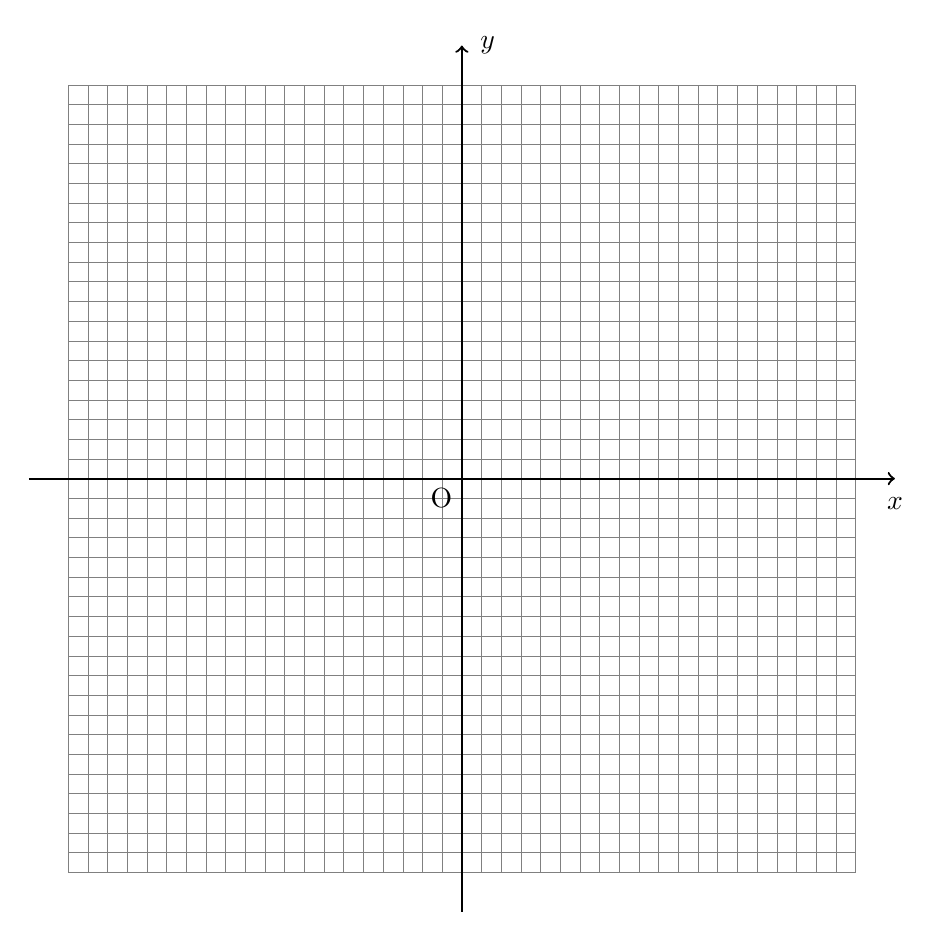
\begin{tikzpicture}
	\draw[help lines, step=0.25] (0,0) grid (10,10);
	\draw (5,5) node[below left]{O};
	\draw[thick, ->] (-0.5,5)--(10.5,5) node[below=3.0] {$x$};
	\draw[thick, ->] (5,-0.5)--(5,10.5) node[right=3.0] {$y$};
	\end{tikzpicture}
	\caption{$xy$平面}
	%\label{fig:quadraticFunction}
\end{figure}
\clearpage